
\section{Use of the API}
\label{key}
In this graph the price change for E.ON can be seen from 2003-01-20 to 2020-11-30:\newline

\begin{figure}[H]
	\centering
	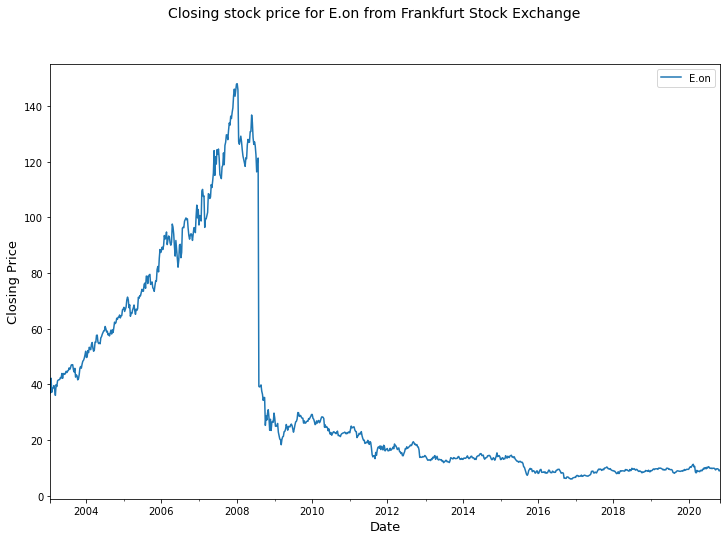
\includegraphics[scale=0.5]{images/Stock_Eon.png}
	\caption{Price of Frankfurt Stock exchange. Source: own depiction.}
	\label{stock}
\end{figure}


\newpage
%comparable firm is not appropriate nor justified

\section{Question 1}
\textit{What are the announcement dates of the three transactions?}
\begin{table}[H]
    \centering
    \begin{tabular}{|l|l|l|}
    \thickhline
         Acquirer & Target & Announcement Date \\\thickhline
         AOT& Time Warner & January 10\textsuperscript{th}, 2000 \\
         AT\&T& Bellsouth& March 6\textsuperscript{th}, 2006\\
        Worldcom& MCI& November 10\textsuperscript{th}, 1997\\ \hline
    \end{tabular}
    \caption{Announcement days}
    \label{aanounce}
\end{table}
\begin{itemize}
    \item AOL and Time Warner announced their merger on Monday, January 10\textsuperscript{th} 2000.
    \item The merger between AT\&T and Bellsouth was announced on a sunday. Therefore, we took the immediately following Monday as the announcement date (March 6\textsuperscript{th} 2006).
    \item The announcement of the Worldcom and MCI merger was November 10\textsuperscript{th} 1997.
\end{itemize}

\section{Question 2}
\textit{Plot the CARs of the portfolio of acquirers and targets, each separately.}\newline
\begin{figure}[H]
    \centering
    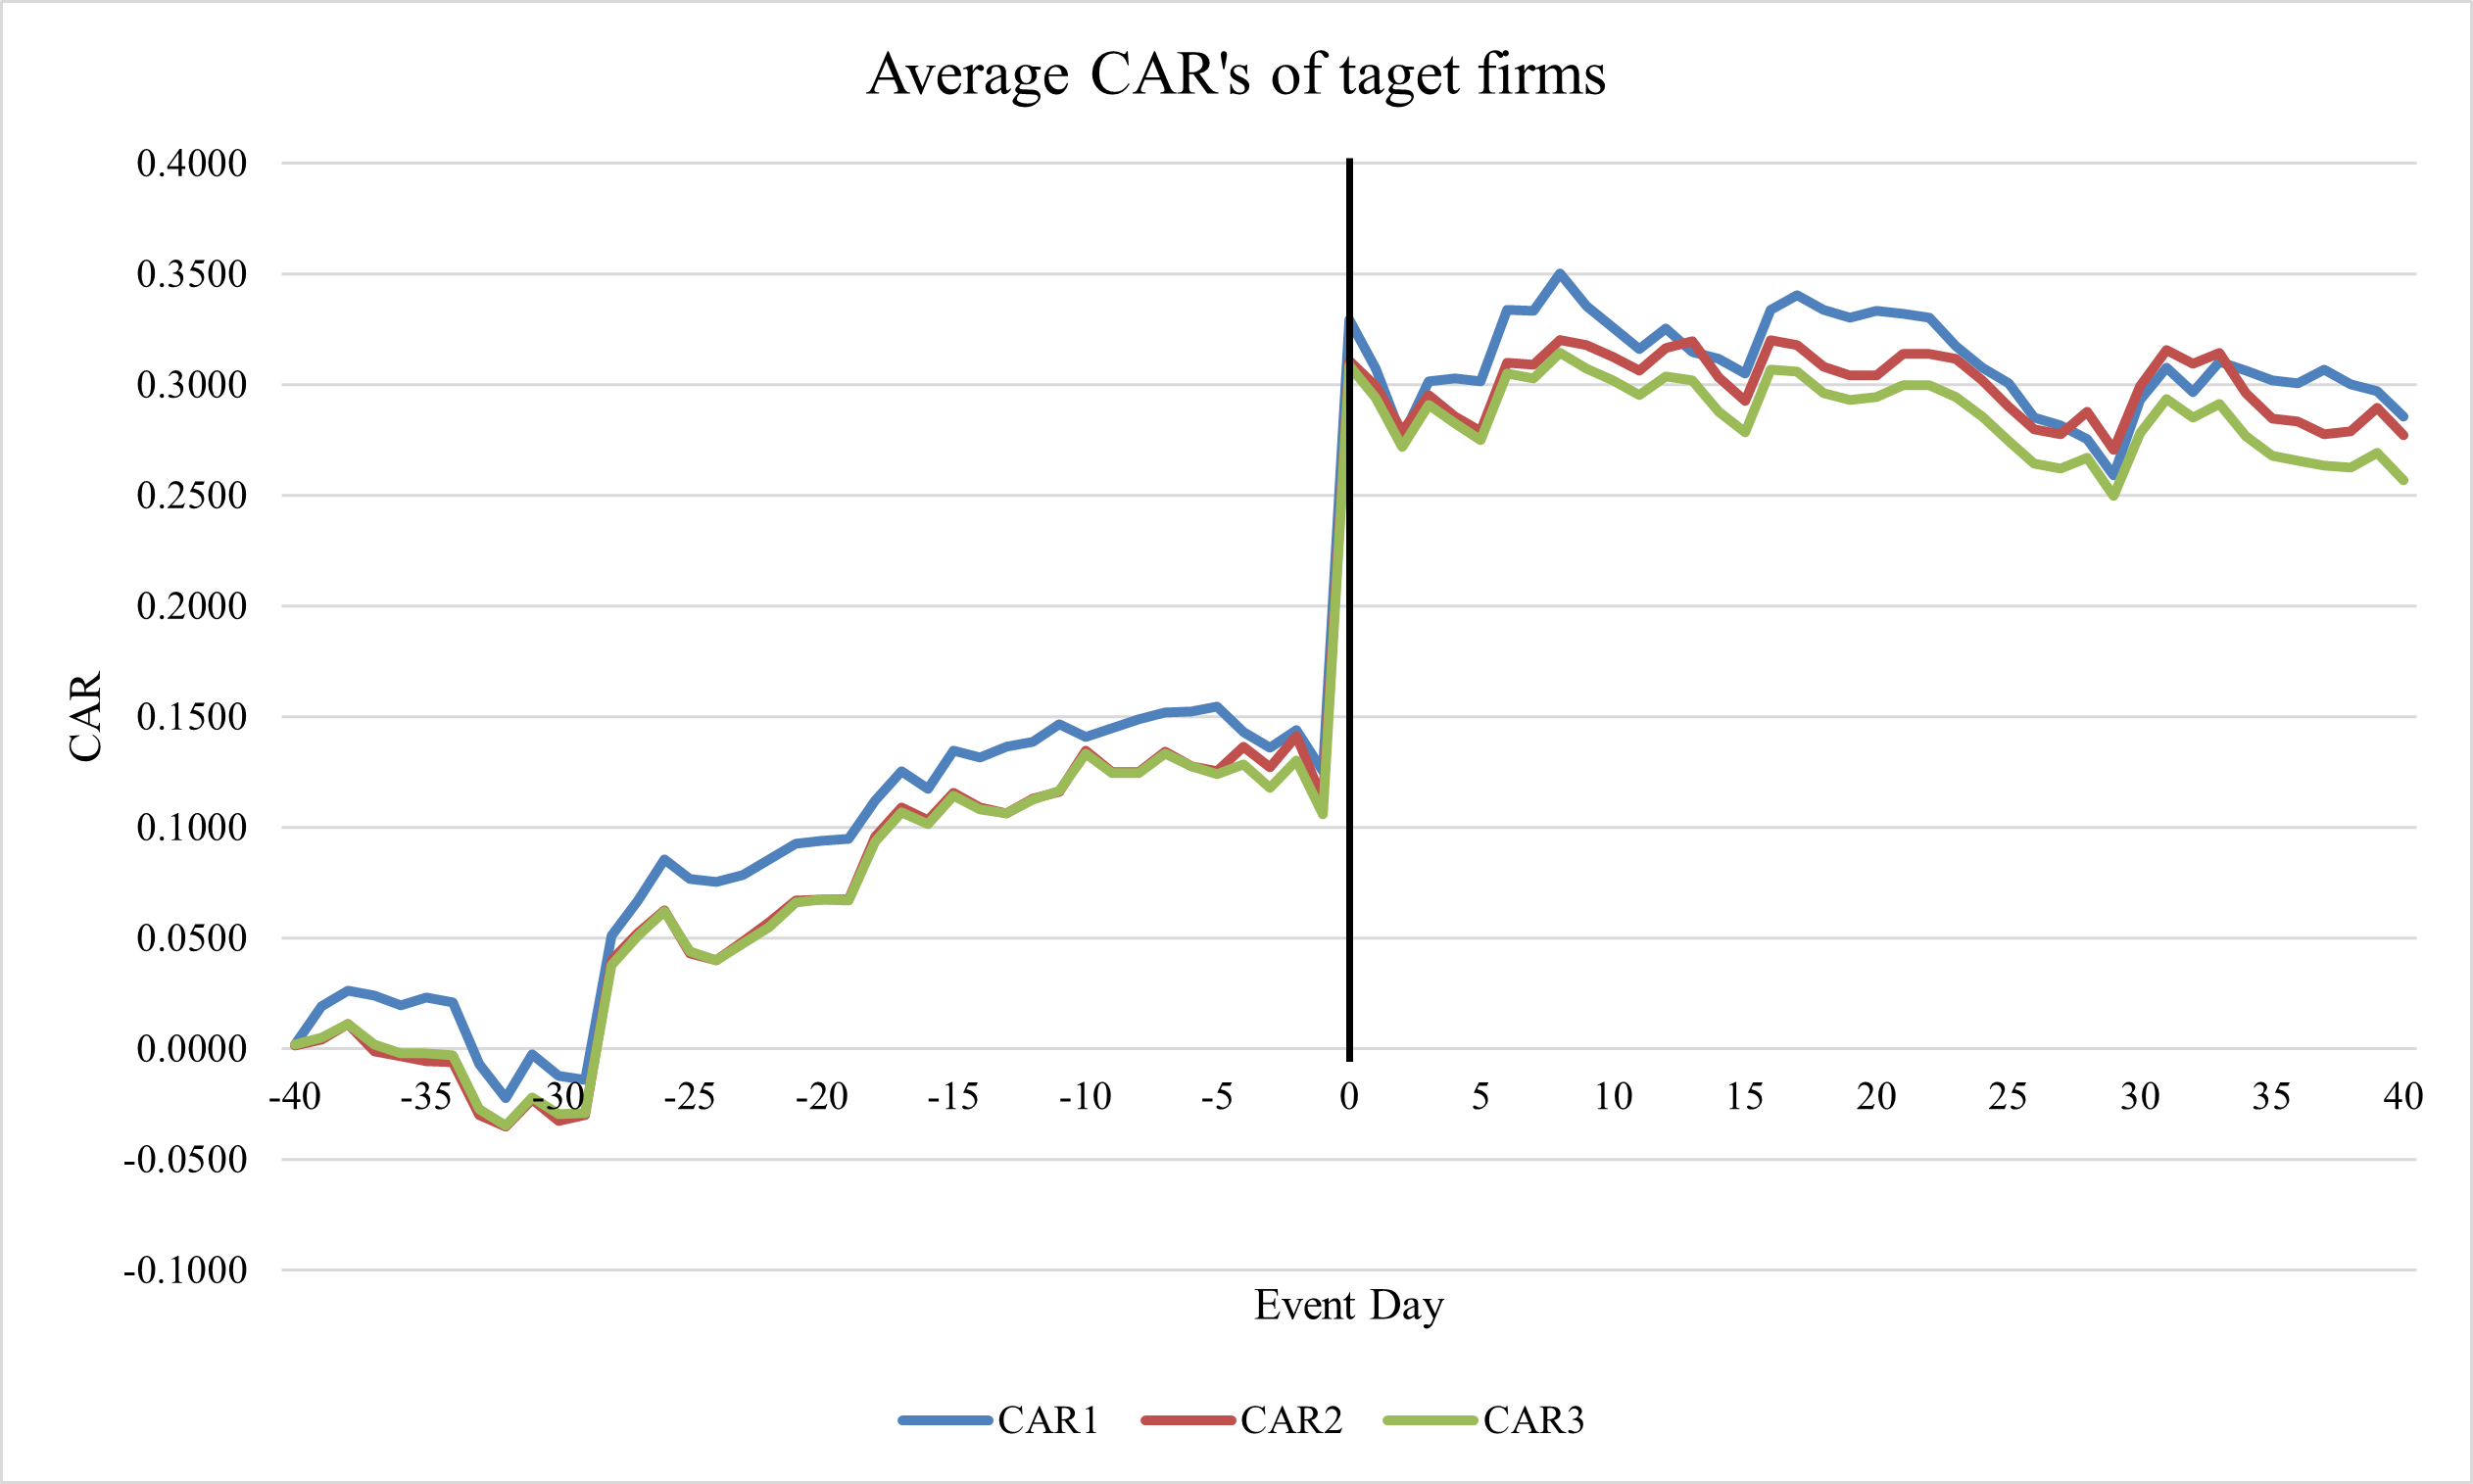
\includegraphics[scale=0.75]{images/Bild1.png}
    \caption{Target firms}
    \label{bildlitargets}
\end{figure}
\begin{figure}[H]
    \centering
    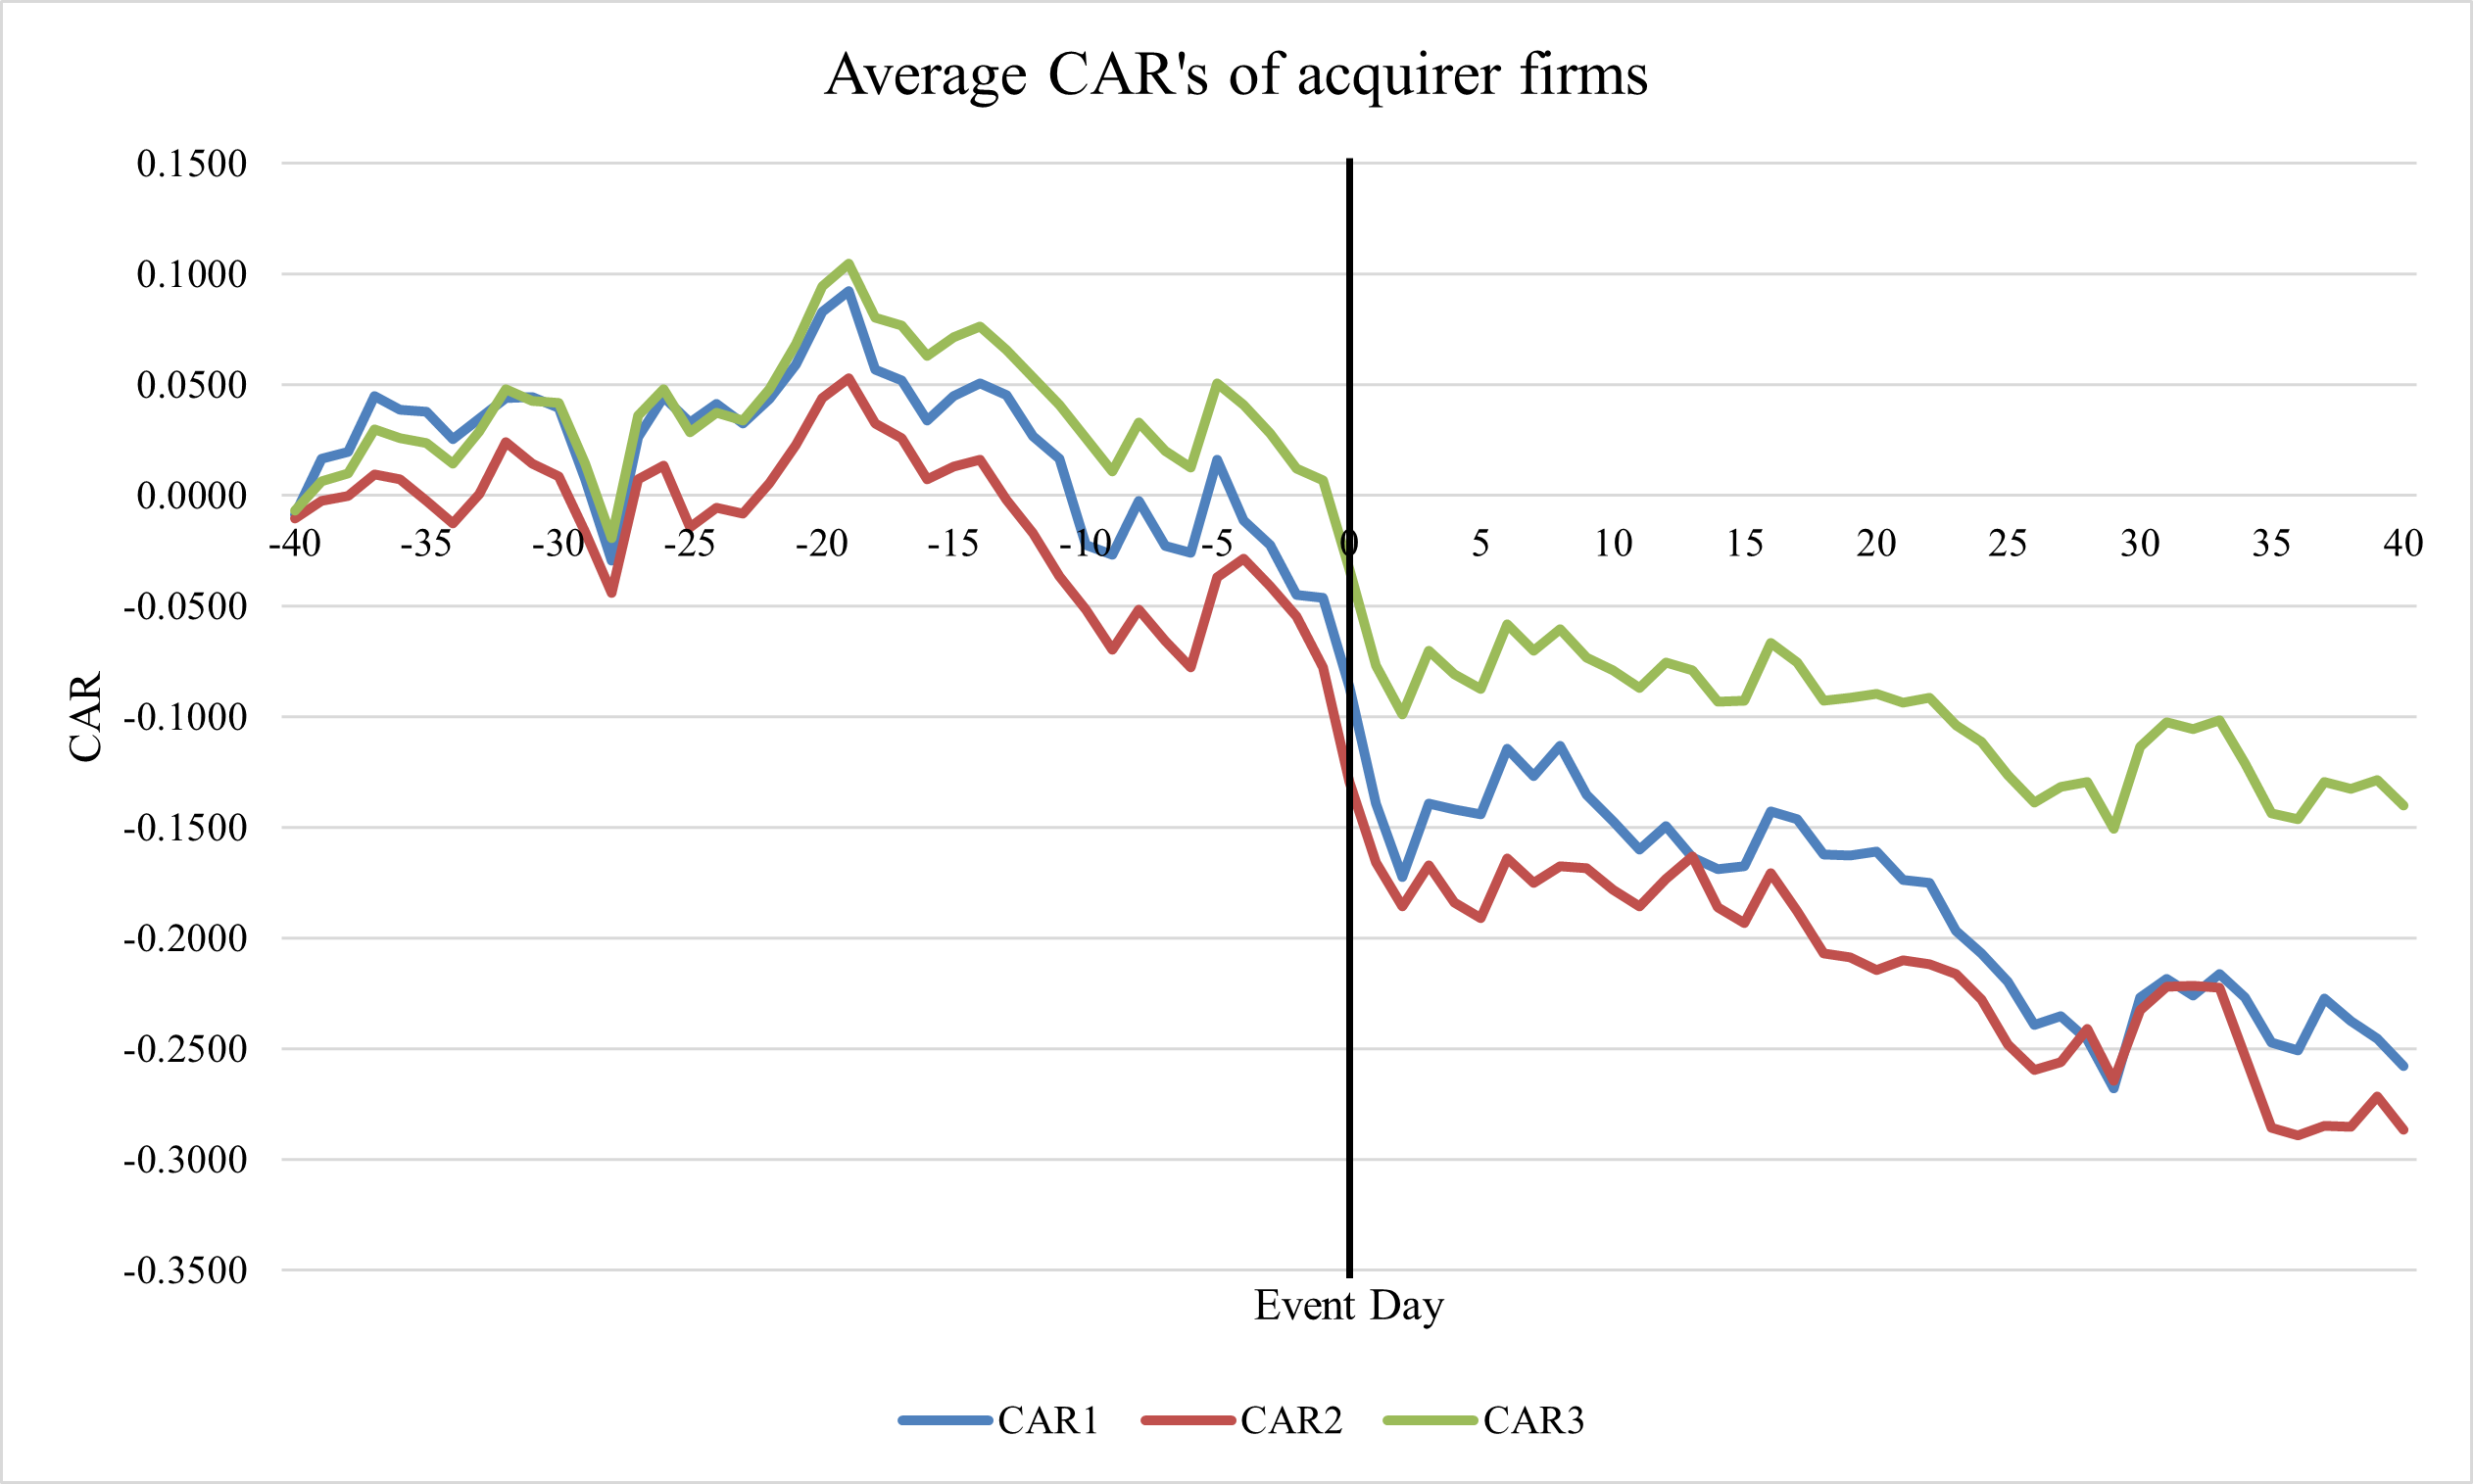
\includegraphics[scale=0.75]{images/Bild2.png}
    \caption{Acquirer firms}
    \label{bildlyacqui}
\end{figure}

\begin{enumerate}[label=\alph*),leftmargin=*]
\item \textit{Interpret the graph for acquirers and the one for targets.} \newline
As we can see in figure \ref{bildlitargets} above, the average cumulative abnormal returns are roughly the same for all three calculation methods for a portfolio of target firms. Only the mean adjusted methods (CAR1) seems to be slightly higher throughout the given time period. Before the announcement day CARs tend to grow which might be due to information leaks or even insider trading. At the merger announcement date, CARs sharply increase implying an offer by the acquirer, which is higher than the actual share price. Afterwards, stock prices of the target firms start a downwards trend. This, might be due to too high expectations of investors or fear of being left out of a good opportunity on the announcement day. Throughout the event window investors gained between 26-28\% more than the benchmarks. \newline
The average CAR’s for the portfolio of acquiring firms tend to fall throughout the event window. Especially on the days $t=0$ to $t=+2$, therefore, right after the announcement, the share prices of the acquiring firms decrease, implied by all three calculation methods. Over the 81 days investors lost between 14-28\% compared to the different benchmarks. \newpage

\item \textit{Plot the CARs of individual targets using the market model for benchmark returns (AR2).} \newline
\begin{figure}[H]
    \centering
    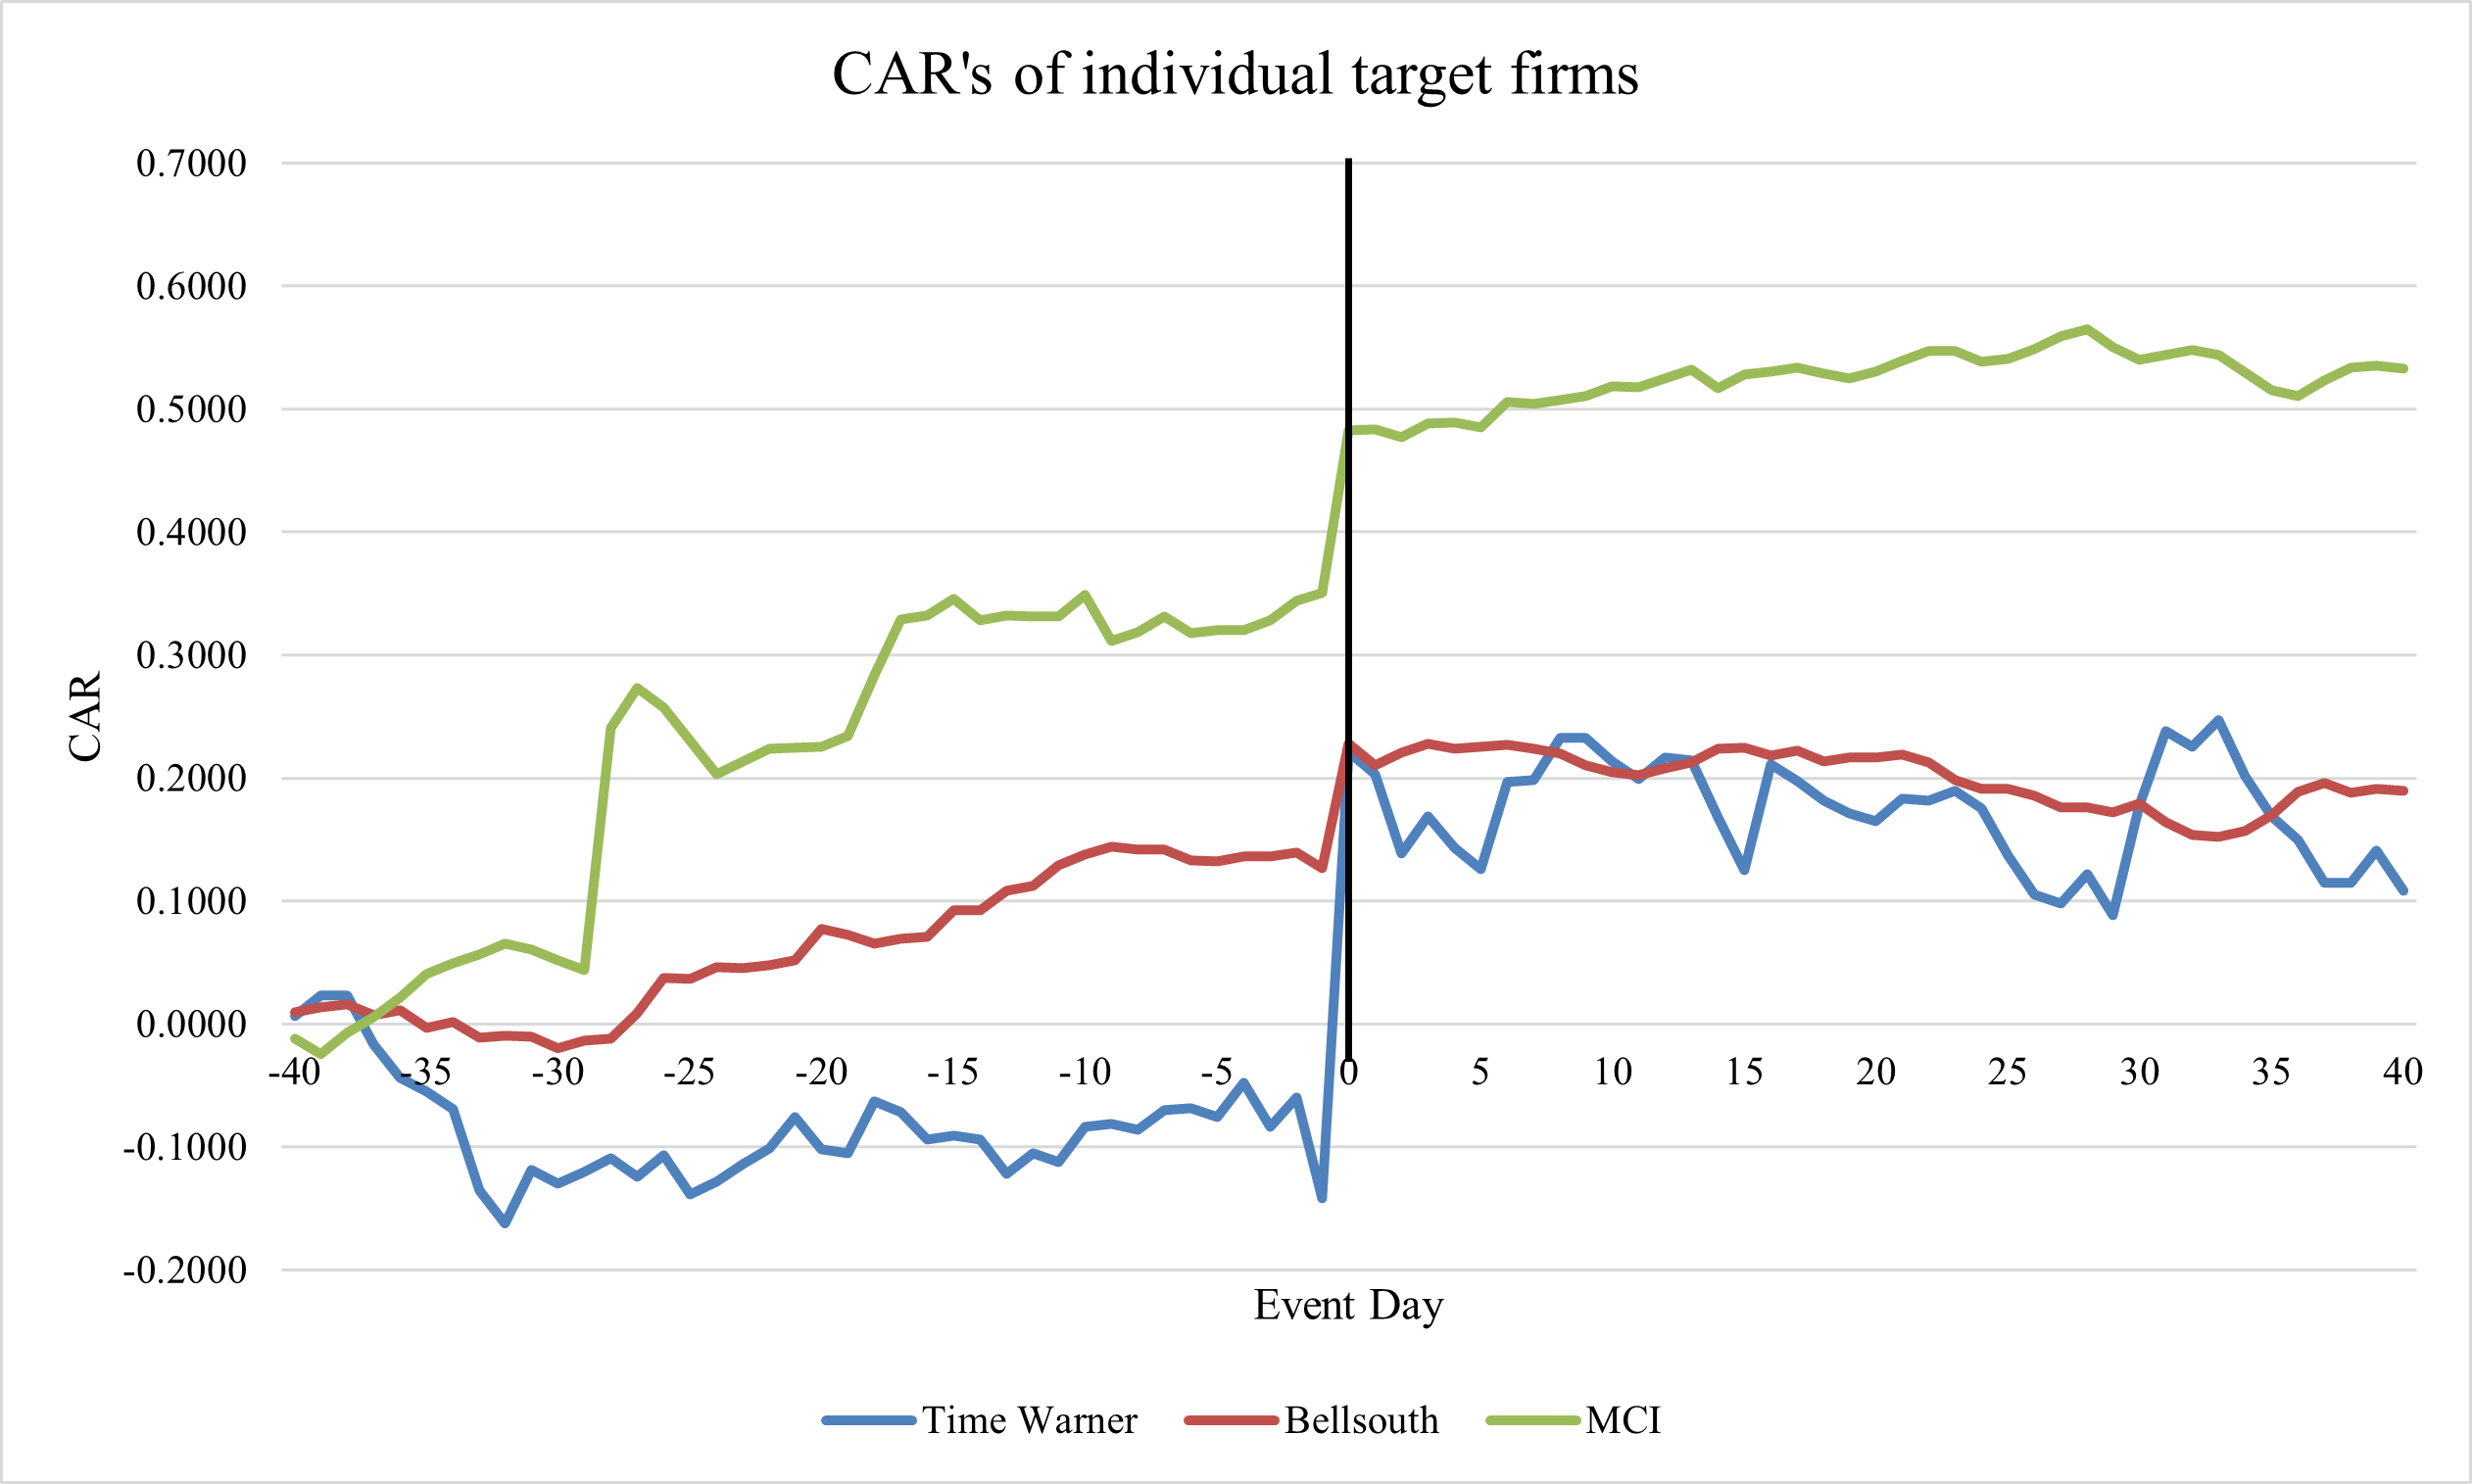
\includegraphics[scale=0.75]{images/Bild3.png}
    \caption{Individual target firms}
    \label{Individualtargetfirm3}
\end{figure}

\item \textit{Did information leak about any of the transactions prior to the announcement day? Explain.} \newline
The graph in figure \ref{Individualtargetfirm3} suggests that no information leaked on the Time Warner transaction. In fact, prior to the announcement date CARs of the company were stable. Bellsouth and MCI, instead shows that some information has been leaking prior to the announcement date, in particular if we look the MCI line. Yet it is most likely that there was an information leak about a possible bid coming up from GTE. Additionally, on October 23, on day $t=-18$ GTE entered into a discussion for a three-way merger between MCI, GTE and themselves, as written in the provided news collection. This led to another sharp increase of CAR's for MCI.\\\\

\item \textit{Plot the CARs of individual acquirers using the market model for benchmark returns (AR2). Interpret!}\\
Cumulative abnormal returns for the acquiring firms using the market model are shown in Figure \ref{aqu}.
While AT\&T goes back to roughly on par with the benchmark after outperforming it by 10\%
following the announcement, Worldcom and AOL especially perform worse than the
benchmark. All three acquiring firms show negative abnormal returns on the day of the merger
announcement, exactly opposite to the target firms.\newline

\begin{figure}[H]
    \centering
    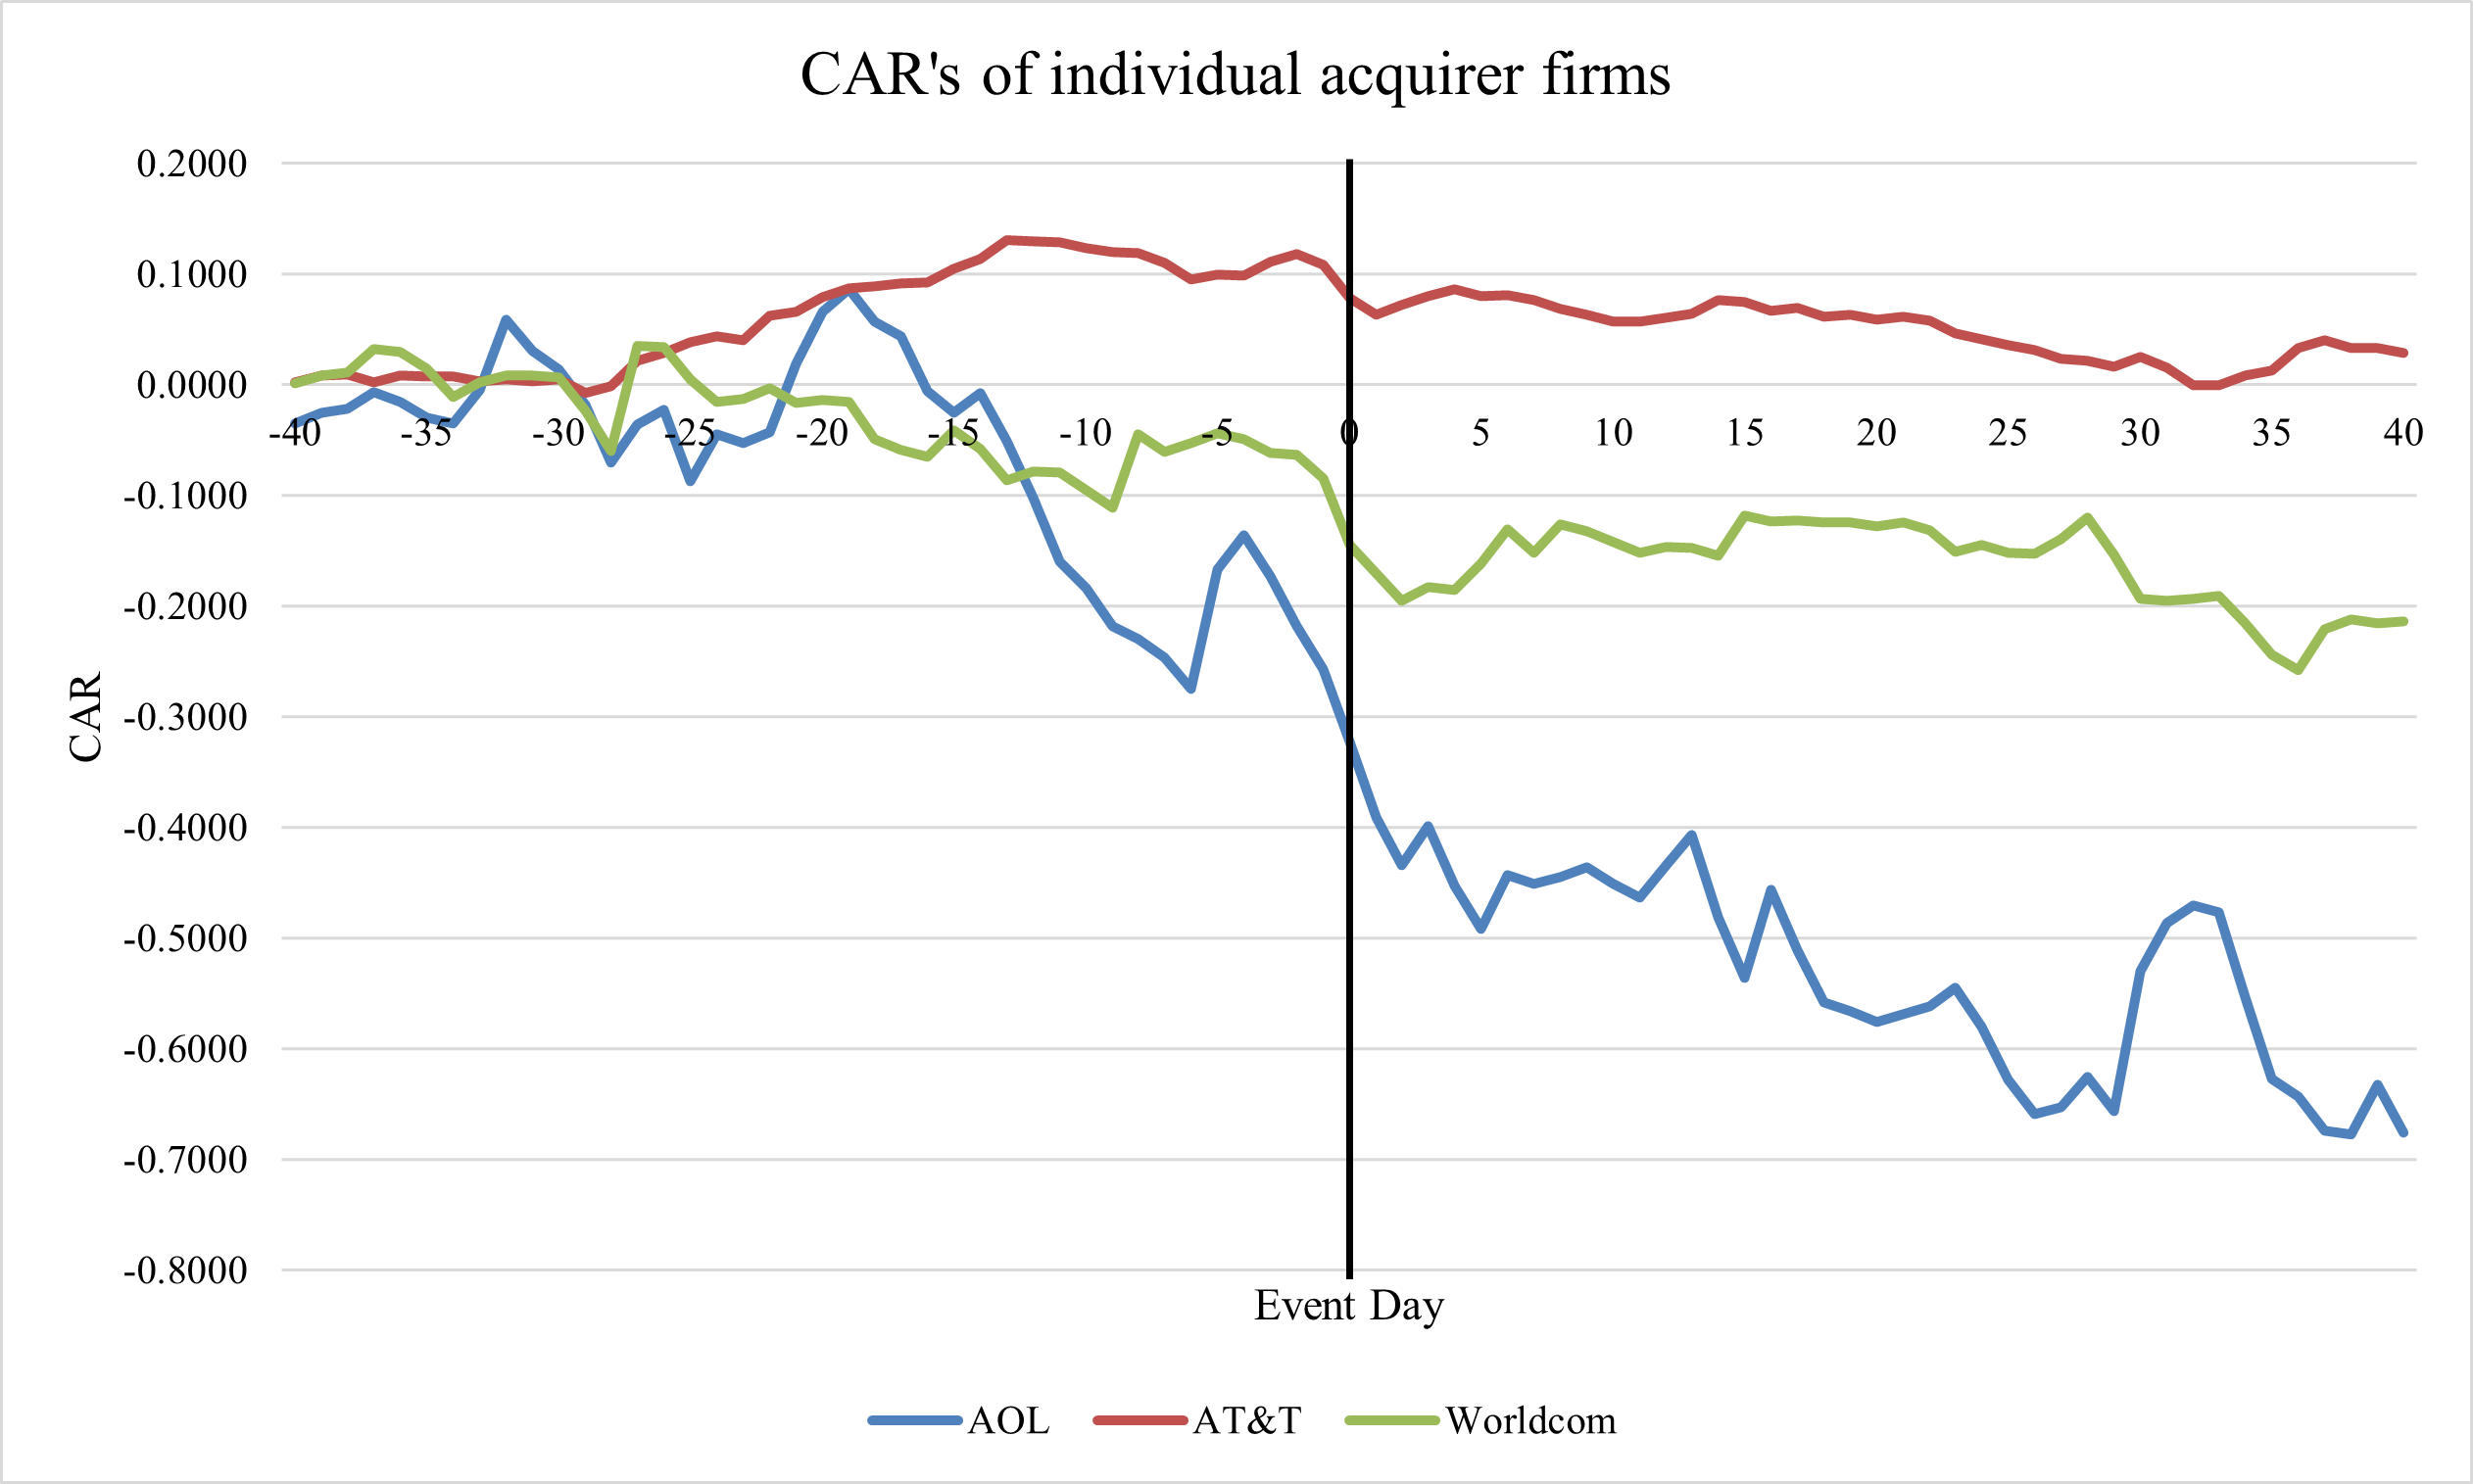
\includegraphics[scale=0.75]{images/Bild4.png}
    \caption{Individual acquirer firms}
    \label{aqu}
\end{figure}
\end{enumerate}


\section{Question 3}
\textit{Are the date t=0 announcement returns statistically significant?} \newline

\begin{table}[H]
\footnotesize
\caption{Abnormal Returns at announcement day}
\label{tab:AbRetAnnouncementDay}
\centering
\begin{tabular}{lcccccc}
\\
\toprule
\multirow{2}*{} & \multicolumn{3}{c}{Targets} & \multicolumn{3}{c}{Acquirers} \\
\cmidrule(lr){2-7}
&\textbf{Time Warner} &\textbf{Bellsouth} &\textbf{MCI} &\textbf{AOL} &\textbf{AT\&T} &\textbf{Worldcom}\\
\midrule 
\textbf{AR1} 	& $0.3902^*$ 	&  $0.0960^*$  	&  $0.1256^*$ 	&$-0.0193$ & $-0.0352^*$ &$-0.0664^*$ \\
t-stat 			& $14.5331$ 	&  $11.5357$  	&  $5.0924$ 	&$-0.4211$ & $-4.5436$ &$-2.8084$ \\
\\
\textbf{AR2} 	& $0.3630^*$ 	&  $0.1013^*$  	&  $0.1319^*$ 	&$-0.0650$ & $-0.0303^*$ &$-0.0602^*$ \\
t-stat 			& $17.3327$ 	&  $14.3134$  	&  $5.7251$ 	&$-1.7990$ & $-4.5957$ &$-2.7291$ \\
\\
\textbf{AR3} 	& $0.3724^*$ 	&  $0.1040^*$  	&  $0.1304^*$ 	&$-0.0340$ & $-0.0273^*$ &$-0.0592^*$ \\
t-stat 			& $17.1503$ 	&  $14.0166$  	&  $5.6578$ 	&$-0.8492$ & $-3.8539$ &$-2.6840$ \\
\bottomrule
&&&&&\multicolumn{2}{l}{\textit{$^*$statistically significant}}\\
\end{tabular}
\end{table}

\begin{enumerate}[label=\alph*),leftmargin=*]
    \item All abnormal returns of the targets are statistically significant (see table \ref{tab:AbRetAnnouncementDay}), given a two sided test with $\alpha=5\%$, regardless of the CAR model used for the computation. For this reason, we reject the null hypothesis that abnormal returns are equal to zero.
    \item As for acquirers, displayed in the last three columns of table \ref{tab:AbRetAnnouncementDay}, at the event day AT\&T as well as Worldcom abnormal returns are statistically significant no matter the CAR computation method, whereas for AOL results are not statistically significant, again, regardless of the CAR method used. Thus, we fail to reject the null hypothesis.
    \item By widening the window by multiple days average abnormal returns most likely wouldn’t be as significant, since the share price usually makes the biggest jump on the day of the merger announcement, given that there was no major information leak following up to the announcement. Therefore, this significant effect would get averaged out over multiple days and most likely lose its significance or at least get less significant.
\end{enumerate}

\section{Question 4}
\textit{Are the date t=-40 to t=+40 CAR’s statistically significant?}\\
Table \ref{Individualtargetfirm3} highlights the Abnormal Returns during the event window for both targets and acquirers.
\begin{enumerate}[label=\alph*),leftmargin=*]
    \item As far as target are concerned, we observe that all are significant except Time Warner, given a two sided test with $\alpha=5\%$. In addition, there is no asymmetry of results between models.
    \item As for acquiring companies, we observe that no one is statistically significant, except for AOL using the market model method for CAR computation. AOL, being an internet company, was particularly affected by the dot-com bubble. For this reason we think that AOL result is biased because the company would have realised an abnormal return independently of M\&A activities.
\end{enumerate}

\begin{table}[H]
\footnotesize
\caption{Abnormal Returns during the event window}
\label{tab:AbRetEventwindow}
\centering
\begin{tabular}{lcccccc}
\\
\toprule
\multirow{2}*{} & \multicolumn{3}{c}{Targets} & \multicolumn{3}{c}{Acquirers} \\
\cmidrule(lr){2-7}
&\textbf{Time Warner} &\textbf{Bellsouth} &\textbf{MCI} &\textbf{AOL} &\textbf{AT\&T} &\textbf{Worldcom}\\
\midrule 
\textbf{CAR1} & $0.1961$ & $0.1933^*$ & $0.4673^*$ & -$0.5283$ & $0.0325$ & $-0.2773$ \\
t-stat & $0.8117$ & $2.5798$ & $2.1067$ & $-1.2806$ & $0.4652$ & $-1.3031$ \\
\\
\textbf{CAR2} & $0.1086$ & $0.1897^*$ & $0.5327^*$ & $-0.6753^*$ & $0.0292$ & $-0.2138$ \\
t-stat & $0.5762$ & $2.9783$ & $2.5693$ & $-2.0777$ & $0.4909$ & $-1.0770$ \\
\\
\textbf{CAR3} & $0.1488$ & $0.1903^*$ & $0.4314^*$ & $-0.3234$ & $0.0280$ & $-0.1245$ \\
t-stat & $0.7615$ & $2.8488$ & $2.0805$ & $-0.8987$ & $0.4405$ & $-0.6271$ \\
\bottomrule
&&&&&\multicolumn{2}{l}{\textit{$^*$statistically significant}}\\
\end{tabular}
\end{table}

\section{Question 5}
\textit{Can we conclude from this sample that, overall, one observes statistically significant abnormal returns around mergers? Explain.}\newline
Given our results, we can confirm statistically significant abnormal returns for the event day on a significance level of 5\% (given a two-tailed test) for five out of the six given firms for all three abnormal return-models. The lowest calculated t-value for these five amounts to -2.2989, thus being generous and taking the maximum amount of degrees of freedom, we get a threshold of 1.96 as critical value to reject the null hypothesis of the abnormal returns being zero. Only AOL’s event day abnormal return is not statistically significant. For the event window only Bellsouth and MCI got statistically significant abnormal returns for all three abnormal return models at a 5\% level. Given this, we argue that we cannot observe statistically significant abnormal returns for the event window.\citep{Bulmash1991}

\section{Question 6}
\textit{How much dollar value was created/destroyed by each of these mergers? Do the calculations based on the entire event window from t=-40 to t=+40.} \newline
We use the following formula to compute the dollar value that was created or destroyed over the event window of 81 days by these mergers:

\begin{equation}
 \Delta W_{40} = CAR_{40} \cdot MV_0   
\end{equation}


\begin{table}[H]
\footnotesize
\caption{Dollar value creation/destruction from mergers (in 1'000 of Dollars)}
\label{tab:AbRetEventwindow_2}
\centering
\begin{tabular}{lcccccc}
\\
\toprule
\multirow{2}*{} & \multicolumn{3}{c}{Targets} & \multicolumn{3}{c}{Acquirers} \\
\cmidrule(lr){2-7}
&\textbf{Time Warner} &\textbf{Bellsouth} &\textbf{MCI} &\textbf{AOL} &\textbf{AT\&T} &\textbf{Worldcom}\\
\midrule 
\textbf{$MV_0$} & $79'826$ & $50'086$ & $15'429$ & $162'057$ & $97'402$ & $31'312$ \\
\\
\textbf{$CAR1_{40}$} & $0.1961$ & $0.1933$ & $0.4673$ & -$0.5283$ & $0.0325$ & $-0.2773$ \\
$\Delta W_{40}$ & $15'655$ & $9'681$ & $7'210$ & $-85'609$ & $3'163$ & $-8'681$ \\
\\
\textbf{$CAR2_{40}$} & $0.1086$ & $0.1897$ & $0.5327$ & $-0.6753$ & $0.0292$ & $-0.2138$ \\
$\Delta W_{40}$ & $8'669$ & $9'502$ & $8'219$ & $-109'440$ & $2'840$ & $-6'695$ \\
\\
\textbf{$CAR3_{40}$} & $0.1488$ & $0.1903$ & $0.4314$ & $-0.3234$ & $0.0280$ & $-0.1245$ \\
$\Delta W_{40}$ & $11'879$ & $9'531$ & $6'657$ & $-52'411$ & $2'731$ & $-3'899$ \\
\bottomrule
\end{tabular}
\end{table}

\section{Question 7}
\begin{enumerate}[label=\alph*),leftmargin=*]

\item \textit{What considerations go into choosing an appropriate event window?} \newline
There is a trade-off between larger and smaller event windows. On one hand, a longer window (>40 days) can capture more merger specific developments like insider trading prior to t=-40 or federal approvals needed for the merger after t=40. On the other hand, as we are comparing the returns of the company to the normal returns in order to detect any abnormal returns, widening the window increases possible benchmark errors. This could result in misleading interpretations. Therefore, the window should not be too small nor too large.
\item \textit{Which benchmark model do you favor and why?}\newline
Out of these three given models we favor the market model. It allows a dynamic estimation of the returns, opposed to a static benchmark from the mean adjusted and market adjusted return models. Additionally, allowing a different exposure to the market in terms of the beta, gives it a more accurate estimation than the market adjusted return model, where we assume no mispricing ($\alpha= 0$) and same volatility of the market for the stock ($\beta= 1$). For an even more precise estimation of the normal return we would suggest considering a multi factor model (e.g. with size, value, interest rates), inspired by the Fama-French three/five-factor model, to decrease the constant alpha.
\item \textit{What is the reason for having days prior to the announcement date in the event window?}\newline
The abnormal returns on the event day may not capture the whole effect of the M\&A event if the market anticipated it or insiders knew of the unannounced transaction.
\item \textit{Why shouldn’t the event and estimation window overlap?}\\
They should not overlap because this would lead the model to be biased. The estimation window is used to estimate the normal returns needed for the CAR computation. Including the event window in the estimation window leads to smaller residuals as we would make an in-sample estimation and thus hinders the capability to measure the true abnormal returns over the event window.\cite{Hardouvelis1987}

\end{enumerate}



\section{Question 8}
\textit{Redo the analysis using a benchmark model that includes the Fama-French factors. Use the following benchmark model:}\newline
\begin{equation}
    R_{j,t} = \alpha_{j} + \beta_{1}MKTRF_{t} + \beta_{2}SMB_{t} + \beta_{3}HML_{t} + \epsilon_{j,t}
\end{equation}

  
Where,$MKTRF$ is the market return less the risk - free rate, $SMB$ is the return difference between small and big stocks and $HML$ is the return difference between high and low market-to-book stocks.


\begin{enumerate}[label=\alph*),leftmargin=*]

\item \textit{Using this benchmark model are the date t=-40 to t=+40 CAR’s statistically significant?}\\

\begin{table}[H]
\footnotesize
\caption{Abnormal Returns during the event window}
\label{ciquee}
\centering
\begin{tabular}{lcccccc}
\\
\toprule
\multirow{2}*{} & \multicolumn{3}{c}{Targets} & \multicolumn{3}{c}{Acquirers} \\
\cmidrule(lr){2-7}
&\textbf{Time Warner} &\textbf{Bellsouth} &\textbf{MCI} &\textbf{AOL} &\textbf{AT\&T} &\textbf{Worldcom}\\
\midrule 
\textbf{CAR1} & $0.1961$ & $0.1933^*$ & $0.4673^*$ & -$0.5283$ & $0.0325$ & $-0.2773$ \\
t-stat & $0.8117$ & $2.5798$ & $2.1067$ & $-1.2806$ & $0.4652$ & $-1.3031$ \\
\\
\textbf{CAR2} & $0.1086$ & $0.1897^*$ & $0.5327^*$ & $-0.6753^*$ & $0.0292$ & $-0.2138$ \\
t-stat & $0.5762$ & $2.9783$ & $2.5693$ & $-2.0777$ & $0.4909$ & $-1.0770$ \\
\\
\textbf{CAR3} & $0.1488$ & $0.1903^*$ & $0.4314^*$ & $-0.3234$ & $0.0280$ & $-0.1245$ \\
t-stat & $0.7615$ & $2.8488$ & $2.0805$ & $-0.8987$ & $0.4405$ & $-0.6271$ \\
\\
\textbf{CAR FFModel} & $0.2151$ & $0.2259^*$ & $0.4179^*$ & $-1.0812^*$ & $0.0590$ & $-0.1250$ \\
t-stat & $1.1626$ & $3.7041$ & $2.0473$ & $-3.7413$ & $1.0195$ & $-0.6372$ \\
\bottomrule
&&&&&\multicolumn{2}{l}{\textit{$^*$statistically significant}}\\
\end{tabular}
\end{table}

Table \ref{ciquee} shows the statistical significance for the targets' and acquirers' CAR Fama French Model for t=40 of the event window given a two sided test with $\alpha=5\%$. The $^*$ marks them in the table 5.  

\item \textit{Compare and contrast this with your answers to question 4.}\\
Given table \ref{ciquee}, by comparing CAR2, calculated by the simple CAPM, with CAR FFModel we see an overall higher t-stat, except for MCI and Worldcom where it decreased.\cite{Bilson2000}


\item \textit{Is this benchmark model superior? Explain}\\

\begin{table}[H]
\footnotesize
\caption{Comparing benchmark models}
\label{sei}
\centering
\begin{tabular}{lcccccc}
	\\
\toprule
\multirow{2}*{} & \multicolumn{3}{c}{Targets} & \multicolumn{3}{c}{Acquirers} \\
\cmidrule(lr){2-7}
&\textbf{Time Warner} &\textbf{Bellsouth} &\textbf{MCI} &\textbf{AOL} &\textbf{AT\&T} &\textbf{Worldcom}\\
\midrule 

\textbf{CAR2 $R^2adj$} & $0.3884$ & $0.2735$ & $0.1219$ & $0.3761$ & $0.2721$ & $0.1248$ \\
\\
\textbf{CAR FFModel $R^2adj$} & $0.4049$ & $0.3273$ & $0.1401$ & $0.5017$ & $0.3023$ & $0.1376$ \\
\bottomrule
\end{tabular}
\end{table}

As we can see from Table \ref{sei} the $R^2adj$, which takes possible overfitting in account, of the FFModel is systematically higher than the one obtained by the CAPM. Therefore, this is a signal of a higher precision of the former when it comes to explain the returns. Additional factors always mean more data is necessary. Obtaining this can sometimes be difficult or increase possible errors due to measuring errors. Nonetheless, we prefer the Fama French Model over the normal CAPM, but would always calculate abnormal returns with several models to get a better overview about the merger.\cite{Abdullah1993}

\end{enumerate}

\section{Question 9}
\begin{itemize}
    \item Improve the formatting of the {\ttfamily.xlsx} file (column/row size, value formats, alignments, grid lines,...). We took the liberty to start to improve it (sorry), hoping that there are no negative consequences on your side.
    \item Let the student think how to get to do the computations in order to answer the required questions, rather than providing the precise guidelines.
\end{itemize}




